% CONFIGURACAO DOCUMENTO
\documentclass[12pt, a4paper]{article}
\usepackage[top=2cm, bottom=1.5cm, left=2.5cm, right=2.5cm]{geometry}
\renewcommand{\baselinestretch}{1.5}
\setlength{\parindent}{1cm}
\usepackage{setspace}
\usepackage{indentfirst}
\usepackage[utf8]{inputenc}
\usepackage[T1]{fontenc}
\usepackage{amsfonts}
\usepackage[brazil]{babel}
\renewcommand{\familydefault}{\sfdefault}
\usepackage{helvet}

% CONFIGURACAO CODIGO
\usepackage{listings}

% CONFIGURACAO REFERENCIAS
\usepackage{natbib}

% CONFIGURACAO IMAGENS
\usepackage{graphicx}

% GERAR TEXTO
\usepackage{lipsum}

\title{APS 5º Semestre}
\author{Daniel Jançanti}
\date{2017}

\begin{document}
	\begin{center}
	\Huge Universidade Paulista\\
	\large Ciência da Computação
	
	\vfill
	
	\large Atividade Prática Supervisionada
	
	\textbf{\MakeUppercase{Desenvolvimento de um sistema para }}
	
	\textbf{\MakeUppercase{reconhecimento de escrita a mão}}
	
	\bigskip
	
	\normalsize{
		Aleksander Rocha - R.A.: C630IH-0\\
		Daniel Jançanti - R.A.: C630IG-2\\
		Ingrid Oliveira - R.A.: C51791-7\\
		Rafaela Aranas - R.A.: C29CII-0\\
	}
	
	\vfill
	
	Araraquara -- \the\year

\end{center}

\thispagestyle{empty}
	\tableofcontents
\thispagestyle{empty}
	\section{Objetivo e motivação do trabalho}
	O objetivo desse trabalho consiste em estudar a comunicação de dados e implementar uma ferramenta para comunicação em rede. Após pesquisa bibliográfica sobre o assunto em questão o grupo deverá criar uma aplicação a qual permita que duas ou mais pessoas possam se comunicar em uma rede, utilizando o protocolo TCP/IP.
	
	A ferramenta será utilizada no seguinte caso: "a empresa fictícia Ambience que faz prevenção de acidentes ambientais resolveu desenvolver uma solução para baratear os custos de ligações telefônicas, essa consiste em um chat de comunicação em rede interna e também online para contato com os interessados".
	
	A ferramenta será implementada na linguagem C\#, e além da comunicação serão acrescidos recursos como login e cadastro de usuário, comunicação um a um e em brodcast onde um usuário envia mensagem para vários, \textit{emoticons}, envio e recebimento de arquivos, etc.
	\section{Introdução}
	Segundo \cite{osorio1991estudo}, um sistema de reconhecimento de caracteres permite que o computador possa adquirir informações através da leitura de textos, ou seja, ao invés de entrar as informações pelo teclado, é possível implementar um sistema computadorizado, associado a um dispositivo ótico, para a aquisição automática de informações descritas sob a forma textual.
	
	Os sistemas de reconhecimento de caracteres possuem uma grande importância junto ao processamento de dados. Isto é, devido ao fato da linguagem escrita ser a forma mais usual do ser humano armazenar e transmitir informações.
	
	As \textbf{redes neurais} são um novo paradigma de desenvolvimento de sistemas, que tem se difundido muito na atualidade. As redes neurais tem se apresentado como uma solução muito adequada para sistemas de reconhecimento de padrões, como é o caso de um sistema de reconhecimento de caracteres, onde os padrões os para serem reconhecidos são os próprios caracteres. Esta característica, a ser demonstrada em maiores detalhes posteriormente, foi o que levou ao estudo e emprego das redes neurais junto a este trabalho.
	
	O \textbf{processamento de imagens} é uma área de estudos da computação que tem crescido muito nos últimos anos. Seu grande crescimento se deve principalmente ao desenvolvimento de equipamentos, cada vez mais sofisticados e baratos, utilizados para a captura e tratamento de imagens digitais. O processamento gráfico engloba as área de processamento de imagem e computação gráfica, onde o processamento de imagens está relacionado ao tratamento e reconhecimento de padrões em imagens, e a computação gráfica está ligada à síntese de imagens e à geração de descrições (dados não pictóricos) utilizadas na obtenção dessas imagens.
	
	O objeto de trabalho no processamento de imagens é a imagem digital, onde esta é definida como sendo uma matriz de M x N elementos (vetores com informações referentes aos pontos da imagem). Cada elemento da imagem digital é denominado de pixel, tendo associado a si uma informação referente à luminosidade e à cor. Esta informação pode ser um valor indicativo de intensidade luminosa. Esta apresentação através de uma matriz bidimensional de pontos é resultante da manipulação da imagem como sendo uma área de memória do computador. A cada pixel é associada uma ou mais posições de memória, as quais deve armazenar as diversas informações referentes a estes. Com isto pode-se armazenar e processar as informações referentes a uma imagem para posteriormente exibi-la.
	
	O \textbf{processo de digitalização} consiste em realizar a aquisição de uma cena, a qual é passada para o computador em um formato adequado para que este possa manupulá-la. As informações visuais são convertidas em sinais elétricos por sensores óticos, e esses sinais são quantificados em valores binários e armazenados na memória do computador. No processo de digitalização, os sinais são amostrados espacialmente e quantificados em amplitude, de forma a obter a imagem digital.
	
	No processo de digitalização, a imagem sofrerá uma amostragem e uma discretização da intensidade luminosa, que é denominada de quantização. No \textbf{processo de quantização}, uma imagem com tons contínuos é convertida em uma de tons discretos. Para o armazenamento e processamento por um computador, cada tonalidade (intensidade da luz refletida por cada ponto da imagem) é representada por um valor armazenado de forma binária. Cada ponto amostrado possuirá portanto um valor binário correspondente à intensidade luminosa da imagem naquele ponto. As imagens podem ser do tipo monocromáticas ou policromáticas. Nas imagens monocromáticas somente uma faixa de comprimentos de onda (uma cor) é analisada pelo sensor, determinando as intensidades de luminosidade para esta faixa. As intensidades de luminosidades descritas acima são denominadas de tonalidades ou níveis de intensidade de cor. Para as imagens policromáticas a digitalização é feita para diferentes faixas de comprimento de onda (diferentes cores).
	\section{Sistemas de reconhecimento de caracteres}
Segundo \cite{silva2003reconhecimento}, os sistemas de reconhecimento ótico de caracteres são sistemas desenvolvidos para, de certa forma, reproduzir a capacidade humana de ler textos.

	\subsection{Origens e Evolução}
	\cite{man1986pattern} disse que as origens da tentativa de sumular a leitura humana datam de 1870, quando foi inventado por Carey, o scanner de retina. A partir da evolução dos dispositivos capazes de captar e traduzir imagens em sinais que podiam ser medidos, novos horizontes foram descobertos. Entretanto, a primeira tentativa bem sucedida de reconhecimento de caracteres foi realizada somente em 1990 pelo cientista russo Tyutin, que desenvolveu um sistema que visava o auxílio de deficientes visuais.
	
	Alguns dos motivos do desenvolvimento de um sistema de reconhecimento de caracteres são:
	\begin{itemize}
		\item Aquisição de dados numéricos comerciais;
		\item Compactação de dados;
		\item Leitura automática de formulários;
		\item Identificação de endereçamento postal;
		\item Reconhecimento de cheques bancários;
		\item Sistemas de aquisição de textos para a tradução automática;
		\item Interface homem x máquina mais natural e sem necessidade de recodificação dos dados (sujeitos a um menor número de erros, pois não é necessário redigitar os textos, introduzindo novos erros);
		\item Auxílio a deficientes visuais, na leitura de textos (tradução e impressão automática em braile)
	\end{itemize}

	\subsection{Tipos de Sistemas de Reconhecimento de Caracteres}
	Os sistemas de reconhecimento de caracteres podem ser desenvolvidos utilizando-se diferentes procedimentos tanto de aquisição de dados como de processamento de informações além de serem orientados para diferentes tipos de aplicações.
	
	Podem ser classificados primeiramente quanto ao tipo de mecanismo utilizado na aquisição dos textos a serem reconhecidos. Nesta categoria, encontram-se os sistemas magnéticos, sistemas mecânicos e sistemas óticos.
	
	Dentro dos sistemas OCR, são encontradas duas classes importantes, aqueles que são baseados no processamento sequencial das informações e os baseados no processamento paralelo. Existem três categorias princiapais: sistema de reconhecimento online, sistema de reconhecimento de caracteres isolados e sistema de reconhecimento de escrito cursiva.
	
	\begin{figure}[!htb]
		\centering
		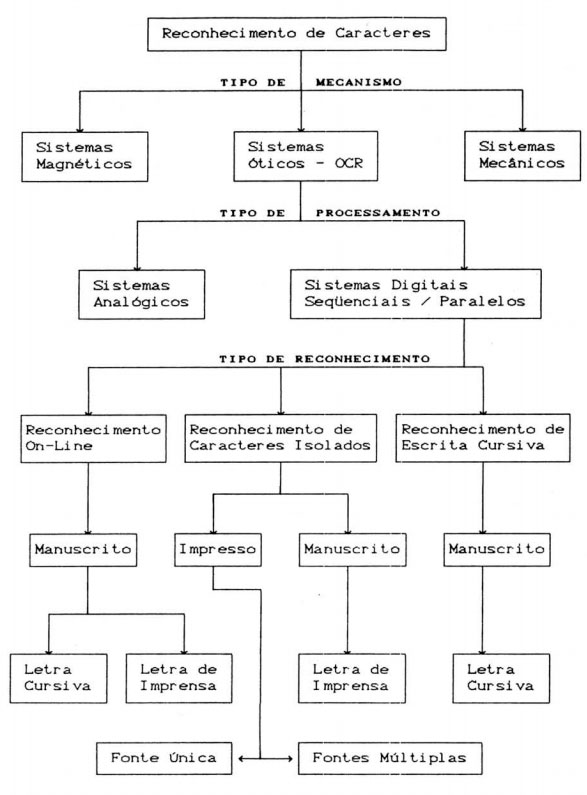
\includegraphics[scale=0.4]{img/organograma-tipos.jpg}
		\caption{Organograma}
		\label{Organograma}
	\end{figure}
	
	\subsection{Descrição dos Sistemas OCR}
	Existem diferentes etapas de processamento das informações visando o reconhecimento de textos por um sistema OCR. Estas etapas se estendem desde a captura da imagem do texto até a obtenção final de uma identificação deste. Em um sistema de COR não se deve considerar apenas a parte referente às técnicas empregadas na resolução do problema de classificação, mas um item de extrema importância é a medicação e avaliação dos resultados obtidos por estes.
		\subsubsection{Etapas de Processamento}
		Em geral, os sistemas de OCR possuem implementadas as seguintes funções: aquisição da imagem do texto, tratamento da imagem, localização e separação dos caracteres, pré-processamento dos padrões, extração de atributos, reconhecimento/classificação dos padrões e pós-processamento.
		
		\begin{figure}[!htb]
			\centering
			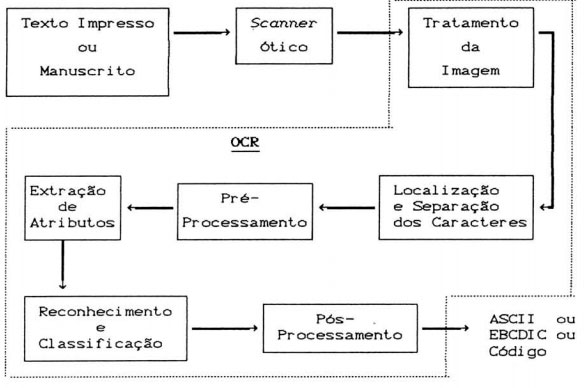
\includegraphics[scale=0.5]{img/etapas-de-processamento.jpg}
			\caption{Etapas do processo de reconhecimento}
			\label{Etapas do processo de reconhecimento}
		\end{figure}
		
		Para a separação dos caracteres, o algoritmo tem que levar em consideração diversos fatores, entre eles: o espaçamento entre caracteres e tamanho do caractere (fixo ou variável), a utilização de uma grade auxiliar (no caso de formulários com espaçamento bem definidos), e o tipo de texto a ser reconhecido, onde podem haver caracteres que se tocam ou caracteres com descontinuidade (características muito importante para módulos de segmentação). Esta etapa de processamento é até hoje uma das etapas mais críticas, sendo um problema ainda não completamente solucionado.
		
		Após terem sido isolados os caracteres, e preferencialmente, com a realização de um ajuste de tamanho e posição pré-definidos, pode-se então realizar uma etapa de extração de atributos. Esta etapada é opcional e dependerá exclusivamente do tipo de técnica empregada no reconhecimento e classificação dos padrões.
		
		\subsubsection{Técnicas de Reconhecimento}
		Existem diferentes técnicas empregadas no reconhecimento de padrões, mas estas podem ser classificadas em três grandes categorias, técnicas baseadas em:
		\begin{itemize}
			\item Atributos globais
			\item Distribuição de pontos e atributos geométricos
			\item Topológicos
		\end{itemize}
	\newpage
\section{Plano de desenvolvimento da aplicação}
Diante de um problema de comunicação frequente entre as pessoas: a questão da agilidade que as informações são transmitidas, pensamos numa solução onde uma única pessoa teria o poder de se comunicar com várias outras de maneira rápida, prática e intuitiva.

Nosso chat vai transmitir dados de um cliente para outro e também de um cliente para vários, tendo que evitar um método retrógrado que seria o uso do telefone. Embora o telefone ainda seja o meio de comunicação mais usado no mundo, ele ainda falha na questão de comunicar várias pessoas ao mesmo tempo.

Baseando-se nessas informações, criamos um meio de comunicação para solucionar essa falha.

Inicialmente a implementação do chat inclui: cadastro de novos usuários, login de usuário, comunicação um para um, comunicação um para muitos e envio de arquivos (documentos, planilhas, fotos, etc), usando o banco de dados mySQL como armazenamento e transmissão de dados por sockets pelo protocolo TCP/IP.
	\section{Projeto}
\lipsum

\begin{figure}[!htb]
	\centering
	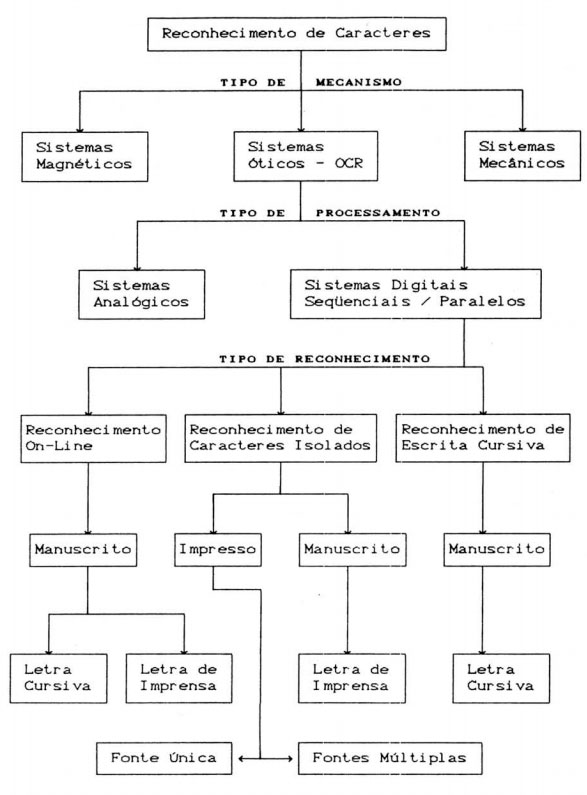
\includegraphics[scale=0.4]{img/organograma-tipos.jpg}
	\caption{Organograma}
	\label{Organograma}
\end{figure}

	
\section{Código fonte}

{\LARGE SERVIDOR}

{\large Servidor-classe-program.cs}
{\scriptsize \lstinputlisting{code/Servidor-Classe-Program.txt} }

{\large Servidor-Classe-QueryReader.cs}
{\scriptsize \lstinputlisting{code/Servidor-Classe-QueryReader.txt} }

{\large Servidor-Classe-TCP.cs}
{\scriptsize \lstinputlisting{code/Servidor-Classe-TCP.txt} }

%{\large Servidor-Transferencia-FT.cs}
%{\scriptsize \lstinputlisting{code/Servidor-Transferencia-FT.txt} }

{\large Servidor-Transferencia-Program.cs}
{\scriptsize \lstinputlisting{code/Servidor-Transferencia-Program.txt} }

{\large Usuario.cs}
{\scriptsize \lstinputlisting{code/Usuario.txt} }

{\large UsuarioControler.cs}
{\scriptsize \lstinputlisting{code/UsuarioControler.txt} }


{\LARGE CLIENTE}

{\large cliente-cadastro.cs}
{\scriptsize \lstinputlisting{code/cliente-cadastro.txt} }

{\large cliente-chat.cs}
{\scriptsize \lstinputlisting{code/cliente-chat.txt} }

{\large cliente-configuracoes.cs}
{\scriptsize \lstinputlisting{code/cliente-configuracoes.txt} }

{\large cliente-enviar-arquivo.cs}
{\scriptsize \lstinputlisting{code/cliente-enviar-arquivo.txt} }

{\large cliente-listeners.cs}
{\scriptsize \lstinputlisting{code/cliente-listeners.txt} }

{\large cliente-login.cs}
{\scriptsize \lstinputlisting{code/cliente-login.txt} }

{\large cliente-main-chat.cs}
{\scriptsize \lstinputlisting{code/cliente-main-chat.txt} }

{\large cliente-md5.cs}
{\scriptsize \lstinputlisting{code/cliente-md5.txt} }


	\include{09_programa}
	\include{10_bibliografia}
\end{document}

1. Capa: identificando o curso, o tema, a relação de alunos do grupo (nome/RA)
2. Índice
3. Objetivo e motivação do trabalho
4. Introdução
5. Fundamentos das principais técnicas biométricas (conceitos gerais)
6. Plano de desenvolvimento da aplicação (elementos e ferramentas utilizadas)
7. Projeto (estrutura e módulos que serão desenvolvidos) do programa
8. Relatório com as linhas de código do programa
9. Apresentação do programa em funcionamento em um computador, apresentando
todas as funcionalidades pedidas e extras.
10. Bibliografia
11. Ficha de Atividades Práticas Supervisionadas